%% Artigo, versão preliminar 1 — baseado no modelo bare_jrnl.tex (IEEEtran V1.8b, Michael Shell).
%% Compilar a partir desta pasta:  pdflatex main && pdflatex main
%% Núcleo independente de framing (benchmark, VLMs para a borda, análise de erros): ao trocar o
%% framing, mudam o título, o resumo e a introdução; as demais seções permanecem.
%% Números transcritos de report/resultados_benchmark_manipulacao.md,
%% report/resultados_benchmark_obstrucao.md, report/analise_fp_fn_manipulacao.md e das saídas de
%% notebooks/benchmark_manipulacao.ipynb (execução completa de 16-17/11/2026); não recalculados aqui.
\documentclass[journal,onecolumn]{IEEEtran}

\usepackage[utf8]{inputenc}
\usepackage[T1]{fontenc}
\usepackage[brazil]{babel}
\usepackage{graphicx}
\usepackage{booktabs}
\usepackage{multirow}
\usepackage{array}
\usepackage{amsmath}
\usepackage{amssymb}
\usepackage{xcolor}
\usepackage{cite}
\usepackage{url}
\usepackage[hidelinks]{hyperref}

\graphicspath{{figures/}}
\newcolumntype{L}[1]{>{\raggedright\arraybackslash}p{#1}}
\newcommand{\Ir}{I_r}
\newcommand{\Ia}{I_a}
% Reduz a tabela à largura da página só quando ela não cabe (nunca amplia).
\newcommand{\fitwidth}[1]{\resizebox{\ifdim\width>\linewidth\linewidth\else\width\fi}{!}{#1}}

\hyphenation{Grounding ViDDAR VIM-Sense}
\renewcommand{\IEEEkeywordsname}{Palavras-chave}

\begin{document}

\title{Reprodução do ViDDAR com VLMs Abertos: Desempenho e Análise de Erros na Detecção de Conteúdo
Prejudicial em RA}

\author{Lucas~Natan~Correia~Couri
        e~Heitor~Mendes~Pereira%
\thanks{Centro de Informática, Universidade Federal de Pernambuco (CIn/UFPE).
E-mails: lncc2@cin.ufpe.br, hmp@cin.ufpe.br.}%
\thanks{Código e documentação: \url{https://github.com/lucascouri2/viddar_rep}.}%
\thanks{Versão preliminar 1, novembro de 2026.}}

\markboth{Versão preliminar 1}{Couri e Pereira: Reprodução do ViDDAR com VLMs abertos}

\maketitle

\begin{abstract}
O ViDDAR usa modelos de visão e linguagem (VLMs) para detectar conteúdo de realidade aumentada (RA)
prejudicial ao usuário: conteúdo virtual que obstrui um objeto real importante ou que distorce o
significado de um objeto real. O sistema foi avaliado apenas com GPT-4o e LLaVA-Next-8B via API, e o
código publicado não permite reproduzir os resultados. Reconstruímos o pipeline de avaliação e o
executamos com cinco VLMs abertos, de 2B a 12B parâmetros, em uma GPU de 12~GB. Com o mesmo VLM do
artigo, os resultados ficam a menos de 4 pontos percentuais dos publicados. Na detecção de obstrução,
em que o VLM só nomeia o objeto e a decisão é geométrica, três modelos chegam a 90,5--91,8\% de
acurácia, no nível do GPT-4o (92,2\%), e os falsos positivos (1,9--6,8\%) vêm todos da escolha do
objeto-chave em cenas ambíguas. Na detecção de manipulação de informação, em que o VLM decide sozinho,
nenhum modelo supera, com o prompt do artigo, o detector trivial que nunca dispara. Propomos um
procedimento de atribuição de erros que usa os rótulos de fator do próprio dataset para separar erros de
conclusão de erros de percepção, medir se o modelo discrimina cada fator e estimar, por oráculo
contrafactual, o ganho máximo de corrigir cada um. Os modelos erram por mecanismos distintos: conclusão
que contradiz as próprias respostas, viés de ``sim'' na percepção e leitura restritiva do fator
semântico. Testamos uma intervenção para cada mecanismo. Tirar a decisão final do VLM é o que mais
ajuda, e leva o melhor modelo a 75,4\% de acurácia; mas só nos modelos que discriminam os fatores, e
nenhum modelo discrimina o fator semântico, que define o ataque.
\end{abstract}

\begin{IEEEkeywords}
Realidade aumentada, modelos de visão e linguagem, segurança, falsos positivos, análise de erros,
replicação.
\end{IEEEkeywords}

\IEEEpeerreviewmaketitle

% =====================================================================================================
\section{Introdução}

\IEEEPARstart{O}{} conteúdo virtual em RA pode prejudicar a tarefa do usuário quando é mal posicionado
ou mal projetado~\cite{sabelman2015,cheng2023}. O ViDDAR~\cite{viddar} detecta dois tipos de conteúdo
prejudicial comparando a imagem crua da câmera com a imagem aumentada: \emph{obstrução}, quando o
conteúdo virtual esconde um objeto real importante, e \emph{manipulação de informação}, quando ele
induz o usuário a interpretar errado um objeto real. Nos dois casos, um VLM é a peça central do
detector.

O artigo avalia o sistema com GPT-4o e com LLaVA-Next-8B, ambos acessados por API. O repositório
público traz o dataset e notebooks de demonstração, mas não o código que gera os resultados, os
baselines ou as métricas. Duas perguntas ficam em aberto: o desempenho se mantém com VLMs abertos
pequenos, executados localmente, como exigiria um sistema que roda na borda? E, quando o detector erra,
\emph{por que} erra? A acurácia agregada não responde à segunda pergunta. Na manipulação, por exemplo,
o modelo de maior acurácia com o prompt do artigo tem a menor taxa de falsos positivos porque quase
nunca detecta um ataque, e dois modelos com a mesma acurácia erram por motivos diferentes.

Este trabalho tem quatro contribuições:
\begin{enumerate}
\item uma reconstrução aberta do pipeline de avaliação do ViDDAR, validada contra o artigo: com o mesmo
  VLM, todos os métodos ficam a menos de 4 pontos percentuais dos valores publicados;
\item um benchmark de cinco VLMs abertos, de 2B a 12B parâmetros, executados localmente em uma GPU de
  12~GB, nas duas tarefas do ViDDAR, com taxas de falsos positivos e negativos, intervalos de confiança
  e testes pareados;
\item procedimentos de atribuição de erros sem anotação nova: na obstrução, por etapa do pipeline; na
  manipulação, por conclusão ou fator, com uma medida de discriminação por fator e um oráculo
  contrafactual que dá o teto de ganho de cada intervenção;
\item a caracterização dos mecanismos de erro e o teste de uma intervenção para cada um (variantes de
  prompt, decisão calculada fora do VLM e alinhamento medido geometricamente), que mostra o que cada
  uma resolve e o que permanece.
\end{enumerate}

% =====================================================================================================
\section{Trabalhos relacionados}

\textbf{Segurança da saída em RA.} O risco de o conteúdo virtual esconder informação real é conhecido
desde os primeiros sistemas de RA~\cite{sabelman2015}. O Arya~\cite{lebeck2017,lebeck2018} propõe um
sistema operacional que aplica políticas sobre a saída, removendo ou tornando transparente o conteúdo
que cobre objetos críticos de classes predefinidas, como pessoas e placas. Davari
\emph{et al.}~\cite{davari2020} tratam a oclusão por colisão com o campo de visão do usuário. Essas
abordagens dependem de cenas ou classes fixadas de antemão; o ViDDAR e seu predecessor
LOBSTAR~\cite{lobstar} substituem essa lista por um VLM que decide, pelo contexto, qual objeto é
importante.

\textbf{Manipulação de informação e de percepção.} Cheng \emph{et al.}~\cite{cheng2023} estudam como
usuários reagem a ataques de manipulação perceptual em realidade mista, e Wang
\emph{et al.}~\cite{wang2024} catalogam padrões manipulativos em RA; ambos são conceituais e não
propõem detectores. O CFIQA~\cite{duan2022} avalia a confusão visual entre conteúdo virtual e real com
métricas de qualidade de imagem, sem julgamento semântico. O ViDDAR modela a manipulação por três
fatores semânticos, e o VIM-Sense~\cite{vimsense}, dos mesmos autores, estende a detecção para pares
de vídeo com raciocínio multimodal.

\textbf{Confiabilidade de VLMs.} Duan \emph{et al.}~\cite{duan2025} mostram que VLMs reconhecem bem
conteúdo virtual \emph{óbvio} em cenas de RA, mas falham em casos sutis. Em geral, VLMs alucinam
objetos e atributos~\cite{tong2024,guan2024} e tendem a responder ``sim'' a perguntas de verificação
de existência~\cite{pope2023}. O próprio ViDDAR usa esse argumento para deixar a decisão de obstrução
a uma regra geométrica, e o VIM-Sense observa que prompts que presumem um usuário facilmente enganável
multiplicam os falsos alarmes do GPT-4o~\cite{vimsense}. Até onde sabemos, nenhum trabalho analisa os
erros desses detectores com VLMs abertos, nem decompõe os falsos positivos da manipulação por fator.

% =====================================================================================================
\section{O ViDDAR}
\label{sec:viddar}

O ViDDAR recebe um par de imagens do mesmo ponto de vista: a imagem crua da câmera, $\Ir$, e a imagem
aumentada vista pelo usuário, $\Ia$ (Fig.~\ref{fig:arch}).

\begin{figure}[!t]
\centering
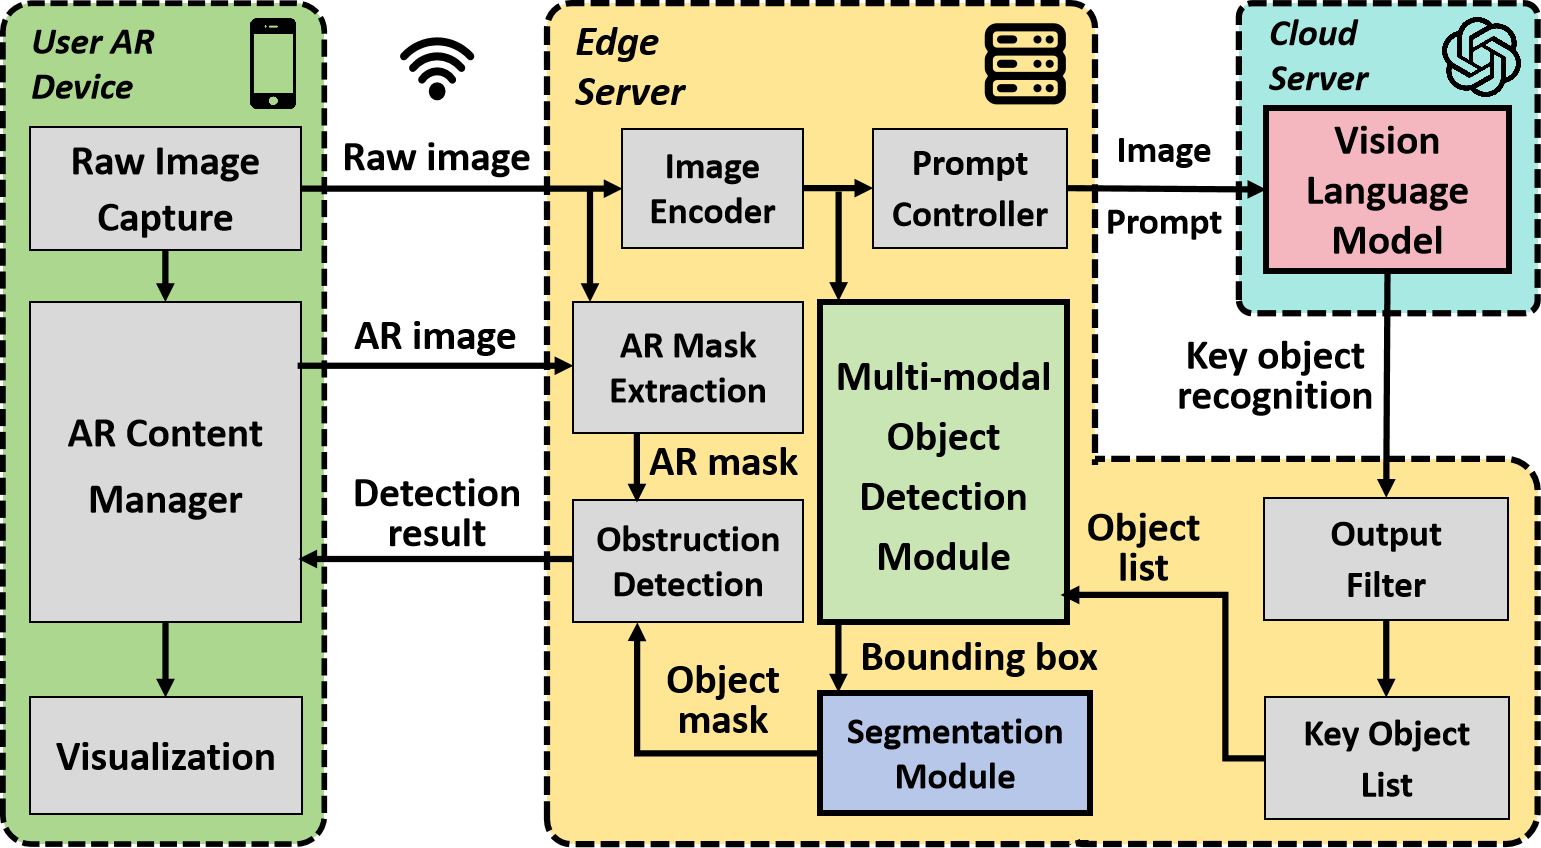
\includegraphics[height=4.3cm]{diagram_obstruction.png}\hfill
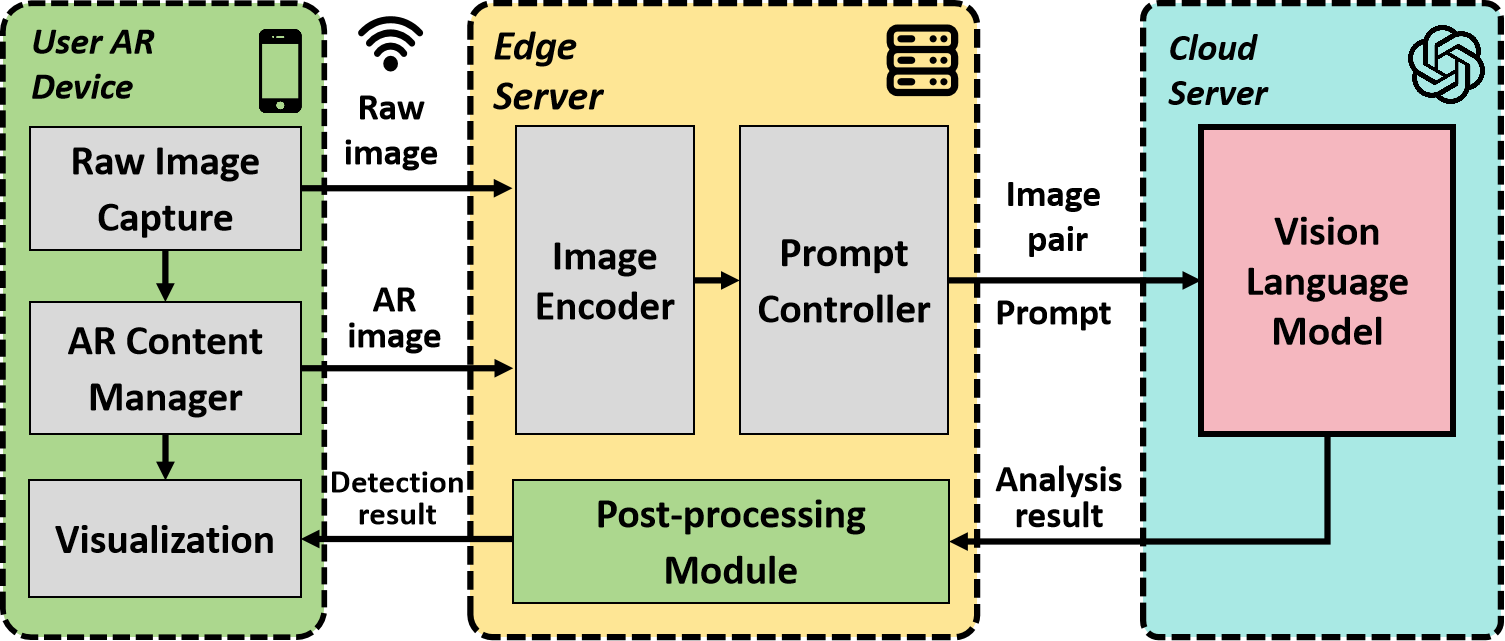
\includegraphics[height=4.3cm]{diagram_information_manipulation.png}
\caption{Arquitetura do ViDDAR para detecção de obstrução (esquerda) e de manipulação de informação
(direita), distribuída entre dispositivo de RA, servidor de borda e nuvem. Fonte: Xiu
\emph{et al.}~\cite{viddar}.}
\label{fig:arch}
\end{figure}

\subsection{Obstrução}
Em $\Ir$ existe um conjunto de objetos-chave $K=\{k_1,\dots,k_n\}$, não predefinido: um objeto é
importante ou não conforme o contexto da cena. Cada $k_i$ tem uma máscara $m_k^i$, e o conteúdo
virtual tem uma máscara $m_c$. Há ataque de obstrução quando
\begin{equation}
O(\Ir,\Ia)=1 \iff \exists\, k_i \in K:\; |m_k^i \cap m_c| \geq \alpha\,|m_k^i|, \qquad \alpha = 0{,}25.
\label{eq:obs}
\end{equation}
O pipeline tem quatro passos: (1) um VLM recebe $\Ir$ e um prompt com atribuição de papel, orientação
de segurança, exemplos e restrição de formato, e devolve o nome do objeto-chave; (2) o Grounding
DINO~\cite{groundingdino} localiza esse objeto a partir do nome; (3) o SAM~\cite{sam} gera a máscara
$m_k$ dentro da caixa detectada; (4) $m_c$ é obtida pela diferença pixel a pixel entre $\Ir$ e $\Ia$,
e a Eq.~\eqref{eq:obs} decide. \textbf{O VLM só nomeia o objeto; a decisão é geométrica.}

O artigo compara o ViDDAR com seis baselines: \emph{end-to-end} (o VLM nomeia o objeto e depois decide,
vendo $\Ir$ e $\Ia$, se ele está obstruído), \emph{underdetailed} (prompt mínimo, sem papel,
orientação de segurança nem exemplos), \emph{greedy} (o VLM lista vários objetos, e há ataque se
qualquer um passar de $\alpha$), mapas de saliência~\cite{hou2007} e de bordas~\cite{canny} sob $m_c$,
e \emph{prior knowledge} (o detector recebe o nome correto do objeto, um limite superior que não usa o
VLM).

\subsection{Manipulação de informação}
Para cada par (objeto real $r_i$, conteúdo virtual $c$), o artigo define três fatores booleanos, que
valem 1 quando a condição é atendida:
\begin{itemize}
\item $A$, \textbf{alinhamento}: o conteúdo está encostado ou preso ao objeto, sem espaço visível;
\item $S$, \textbf{estilo}: textura, cor e iluminação realistas, que misturam o conteúdo à cena;
\item $I$, \textbf{informação}: a combinação faz o usuário acreditar que o objeto tem uma função ou
  informação que não tem, ou esconde uma que tem.
\end{itemize}
Há ataque quando os três valem ao mesmo tempo:
\begin{equation}
M(\Ir,\Ia)=1 \iff \exists\, (r_i,c): A_i \wedge S_i \wedge I_i .
\label{eq:man}
\end{equation}
Basta um fator valer 0 para o par ser benigno: um conteúdo enganoso mas desalinhado, por exemplo, é
percebido como virtual e não engana.

Na prática, o VLM recebe $\Ir$ e $\Ia$ com um questionário de seis perguntas: (1) qual é o conteúdo
virtual; (2) qual objeto real interage com ele; (3)--(5) as perguntas sobre $A$, $S$ e $I$, cada uma
respondida com ``yes'' ou ``no'' e uma justificativa; e (6) a conclusão, com a instrução de responder
``yes'' só se as respostas 3, 4 e 5 forem ``yes''. \textbf{A decisão do sistema é o ``yes'' ou ``no''
que aparece por último na resposta}, ou seja, a conclusão da pergunta 6, e não a Eq.~\eqref{eq:man}
aplicada às respostas 3--5. Duas instruções do prompt favorecem respostas positivas: ele afirma que
$\Ia$ foi criada adicionando conteúdo virtual, e a pergunta 5 pede ao modelo que ``pense
criativamente'' e só responda ``no'' se a combinação não tiver relação semântica específica.

\subsection{Resultados publicados}
Com GPT-4o, o artigo relata 92,15\% de acurácia na obstrução e 82,46\% na manipulação. Com
LLaVA-Next-8B~\cite{llava}, os valores são 89,21\% e 42,98\%; o artigo observa que o LLaVA rotula quase
tudo como manipulação.

% =====================================================================================================
\section{Reconstrução do pipeline}
\label{sec:impl}

O repositório dos autores contém o dataset, dois notebooks de demonstração com GPT-4o e os
questionários do estudo com usuários, sem as respostas. Não havia código para outros VLMs, para os
seis baselines, para as métricas de reconhecimento do objeto-chave e de segmentação, nem para gerar as
máscaras de conteúdo virtual: só 32 máscaras foram publicadas, sem indicação de a qual par pertencem.
Os notebooks também divergem do artigo em pontos que afetam o resultado; o de obstrução, por exemplo,
sorteia $\alpha$ entre 0,175 e 0,225 a cada imagem e repete a consulta quando a resposta contém certas
palavras.

Reimplementamos o pipeline seguindo o artigo. São iguais ao artigo a Eq.~\eqref{eq:obs} com o mesmo
$\alpha$, os prompts (transcritos literalmente), os seis baselines, o segmentador e a regra de decisão
da manipulação. Onde o artigo é omisso, tomamos uma decisão explícita e configurável
(Tabela~\ref{tab:decisoes}). Duas diferenças são impostas: o Grounding DINO 1.5 do artigo só existe
via API fechada, então usamos a versão aberta; e os VLMs são modelos abertos executados localmente.

Acrescentamos, sem alterar as decisões do artigo: a razão de obstrução salva por amostra, que permite
recalcular qualquer $\alpha$; a extração das respostas 3--5 da manipulação como previsões de $A$, $S$ e
$I$, com o recálculo da Eq.~\eqref{eq:man}; e métricas adicionais (Seção~\ref{sec:protocolo}). Toda
resposta bruta do VLM é guardada, de modo que limiares, regras de decisão e métricas podem ser
recalculados sem consultar o modelo de novo.

\begin{table}[!t]
\renewcommand{\arraystretch}{1.2}
\caption{Decisões de implementação onde o artigo é omisso ou inviável de seguir}
\label{tab:decisoes}
\centering
\footnotesize
\begin{tabular}{L{3.6cm}L{4.6cm}L{7.0cm}}
\toprule
Item & Artigo & Nossa implementação \\
\midrule
Máscara $m_c$ & ``comparando $\Ir$ e $\Ia$ no nível de pixel'' & diferença $>30$ em algum canal RGB, abertura $3\times3$ e fechamento $7\times7$; IoU mediano de 0,99 com as 32 máscaras publicadas \\
Detector & Grounding DINO 1.5 (API fechada) & Grounding DINO base aberto; limiares de caixa 0,3 e de texto 0,25; caixa de maior confiança, como no notebook \\
Objeto não detectado & não informado & razão 0, ou seja, ``não obstruído'' \\
Decodificação & não informada & greedy (temperatura 0) \\
Resolução & GPT-4o com \emph{detail: high} & imagens reduzidas a até 1 megapixel \\
Retentativas & o notebook repete a consulta se a resposta contém ``sorry'', ``however'' etc. & nenhuma: com decodificação greedy a resposta seria a mesma, e o filtro enviesa o resultado \\
Acerto do objeto-chave & critério não publicado & léxico (sinônimos da classe) e \emph{grounded} (IoU $\geq 0{,}5$ com a máscara verdadeira); as conclusões usam o \emph{grounded} \\
Fatores $A$, $S$, $I$ & não extraídos & primeiro ``yes''/``no'' de cada resposta 3--5 \\
\bottomrule
\end{tabular}
\end{table}

% =====================================================================================================
\section{Protocolo experimental}
\label{sec:protocolo}

\subsection{Dados}
Usamos o dataset publicado com o ViDDAR. A obstrução tem 306 pares de 23 classes de objeto-chave (145
obstruídos e 161 não obstruídos), com máscaras dos objetos e rótulo de obstrução. A manipulação tem 114
pares, de 10 combinações de conteúdo virtual e objeto real, com os rótulos $A$, $S$, $I$ e $M$.

Antes dos experimentos, verificamos a consistência do dataset:
\begin{itemize}
\item os rótulos de manipulação satisfazem $M=A\wedge S\wedge I$ nos 114 pares;
\item as máscaras $m_c$ derivadas para os 306 pares coincidem com as 32 publicadas (IoU mediano de
  0,99);
\item com as máscaras verdadeiras dos objetos-chave, os rótulos de obstrução são mais bem explicados por
  $\alpha\approx 0{,}2$ (98,4\% de concordância) do que pelo $\alpha=0{,}25$ do artigo (94,1\%).
\end{itemize}

A Tabela~\ref{tab:composicao} mostra a composição da manipulação. \textbf{Quase todo par benigno tem
dois dos três fatores verdadeiros}: os negativos foram construídos sobretudo com desalinhamento (34
pares) ou textura artificial (27), e só 11 são benignos por não sugerirem nada falso ($I=0$). Para
acertar um benigno, o modelo precisa negar exatamente o fator que falha, o que torna o dataset
particularmente sensível a um viés de ``sim''. Um detector trivial, que nunca dispara, acerta 61,4\%
dos pares (70/114).

\begin{table}[!t]
\renewcommand{\arraystretch}{1.15}
\caption{Composição do dataset de manipulação pelos rótulos verdadeiros dos fatores}
\label{tab:composicao}
\centering
\footnotesize
\begin{tabular}{cccL{7.2cm}cc}
\toprule
$A$ & $S$ & $I$ & O que acontece no par & Pares & $M$ \\
\midrule
1 & 1 & 1 & alinhado, realista e enganoso & 44 & 1 \\
0 & 1 & 1 & realista e enganoso, mas desalinhado & 32 & 0 \\
1 & 0 & 1 & alinhado e enganoso, mas com textura artificial & 25 & 0 \\
1 & 1 & 0 & alinhado e realista, mas não sugere nada falso & 11 & 0 \\
0 & 0 & 1 & enganoso, mas desalinhado e com textura artificial & 2 & 0 \\
\midrule
 & & & Total & 114 & 44 ataques \\
\bottomrule
\end{tabular}
\end{table}

\subsection{Modelos e execução}
Avaliamos cinco VLMs abertos que cabem em 12~GB e aceitam duas imagens por conversa:
Qwen3-VL-2B e Qwen3-VL-4B~\cite{qwen3vl} em bf16; e, quantizados em 4 bits (NF4~\cite{qlora}),
Qwen3-VL-8B, LLaVA-Next-8B (o modelo do artigo) e Gemma~4~12B~\cite{gemma4}. Os três Qwen mostram o
efeito do tamanho dentro de uma família; LLaVA e Gemma trazem outras arquiteturas. Todos rodam em uma
NVIDIA RTX 3060 de 12~GB, com decodificação greedy, imagens reduzidas a até 1 megapixel (o processador
do Gemma usa um orçamento fixo de 280 tokens por imagem) e $\alpha=0{,}25$. Os modelos são carregados
um de cada vez: o VLM é descarregado da memória antes do Grounding DINO e do SAM.

O custo por amostra é de 1 a 2~s na etapa de VLM da obstrução, mais 0,8~s de detecção e segmentação, e
de 13 a 21~s por par na manipulação com o questionário do artigo. Os resultados do artigo com GPT-4o
servem apenas como referência: não temos as respostas dele par a par.

\subsection{Intervenções na manipulação}
\label{sec:intervencoes}
Além do prompt do artigo (\texttt{paper}), avaliamos variantes escritas a partir das definições do
artigo, cada uma ligada a uma hipótese sobre a origem dos erros:
\begin{itemize}
\item \texttt{neutral}: a imagem aumentada ``pode conter'' conteúdo virtual, e sai o ``pense
  criativamente''. Hipótese H1: o prompt induz um viés de ``sim'';
\item \texttt{definition}: a pergunta 5 começa com a definição de $I$ da Seção~3.2 do artigo, que
  inclui adições plausíveis. Hipótese H3: o modelo lê $I$ de forma restritiva;
\item modo decomposto (\texttt{paper\_decomposed}, \texttt{definition\_decomposed}): quatro chamadas
  por par (conteúdo e objeto, depois $A$, $S$ e $I$ separados), com a decisão $A\wedge S\wedge I$
  calculada em código. Hipótese H2: a conclusão se desconecta das respostas, e cada resposta
  contamina as outras.
\end{itemize}
Avaliamos também um \textbf{alinhamento geométrico} (C2), que substitui a resposta do VLM sobre $A$ por
uma medida em pixels: $m_c$ vem da diferença de pixels, como na obstrução; o objeto citado pelo VLM é
localizado pelo Grounding DINO e segmentado pelo SAM em $\Ir$; e a medida é a menor distância entre as
duas máscaras, normalizada pelo tamanho do conteúdo. O limiar é escolhido por validação cruzada
estratificada em 5 partições, nunca no conjunto inteiro, e a decisão híbrida é
$A_{\text{geo}}\wedge S_{\text{VLM}}\wedge I_{\text{VLM}}$. Todas as variantes ficam ao lado da decisão
do artigo, que continua sendo a métrica principal.

\subsection{Métricas}
Além das métricas do artigo (acurácia, precisão e recall), reportamos:
\begin{itemize}
\item as taxas de falsos positivos (FPR, a fração de pares sem ataque classificados como ataque) e de
  falsos negativos (FNR), com intervalos de confiança de 95\% de Wilson~\cite{wilson};
\item a acurácia balanceada, $(\text{recall}+\text{especificidade})/2$, que vale 50\% em qualquer
  detector constante e permite comparar detectores que disparam muito com os que quase não disparam;
\item o teste de McNemar exato nos mesmos pares, com $p<0{,}05$, para comparar variantes, modelos e
  cada execução com o detector trivial.
\end{itemize}
Respostas que não podem ser interpretadas contam como erro; foram no máximo 2 por execução. Com 114
pares de manipulação, diferenças de poucos pontos percentuais não são significativas.

% =====================================================================================================
\section{Resultados: obstrução}
\label{sec:obs}

A Tabela~\ref{tab:obs} traz os resultados. \textbf{A replicação confere com o artigo:} com o LLaVA, o
ViDDAR e o \emph{end-to-end} ficam a 1,0 e 3,9 pontos dos valores publicados, e os métodos que não
usam VLM também coincidem (\emph{prior knowledge} 93,8\% contra 93,1\%; saliência e Canny perto do
acaso). Isso valida detector, segmentação, máscara $m_c$ e Eq.~\eqref{eq:obs}. A troca do Grounding
DINO 1.5 pela versão aberta não prejudicou a segmentação (mIoU de 85,1\% contra 78,8\% no \emph{prior
knowledge}).

\textbf{A partir de 4B parâmetros, a escolha do VLM importa pouco.} Qwen3-VL-4B, Qwen3-VL-8B e Gemma
empatam entre si (McNemar, $p\geq 0{,}39$) e ficam a 0,4--1,7 ponto do GPT-4o. O 4B e o 8B não se
distinguem nem do \emph{prior knowledge} ($p=0{,}065$ e $0{,}15$): com eles, reconhecer o objeto-chave
deixa de ser o gargalo do pipeline. O 2B perde para todos ($p\leq 0{,}001$). Dentro da família Qwen, o
tamanho ajuda do 2B para o 4B (+6,9 pontos), mas não do 4B para o 8B. O detector erra mais por omissão
que por alarme falso: FPR de 1,9\% a 6,8\% e FNR de 13,8\% a 24,8\%.

\textbf{A decisão geométrica é o que torna o detector robusto.} Nos cinco modelos, o ViDDAR supera o
\emph{end-to-end}, em que o VLM decide sozinho, por 8,8 a 39,5 pontos ($p\leq 0{,}001$). No
\emph{end-to-end}, cada modelo tem um viés próprio: o 2B diz ``obstruído'' em 259 de 306 amostras (FPR
de 87,6\%), o LLaVA em só 28 (recall de 8,3\%), o 8B tende ao ``sim'' e o 4B ao ``não''. O Gemma é a
exceção: diz ``sim'' em 145 amostras, exatamente o número de obstruídas, e seu \emph{end-to-end}
(81,7\%) iguala o do GPT-4o no artigo.

\textbf{O prompt do objeto-chave é parte do método.} Sem a orientação de segurança e os exemplos
(\emph{underdetailed}), quatro dos cinco modelos perdem de 5,5 a 10,4 pontos, como no artigo. Os
modelos passam a nomear objetos salientes, mas irrelevantes: ``door'' é a resposta mais frequente do
Gemma (29 vezes) e do 2B (27), e o reconhecimento do Gemma cai de 88,6\% para 62,1\%. O \emph{greedy}
empata com o ViDDAR, exceto no 2B, em que listar vários objetos compensa a má escolha de um único
(+4,3 pontos, $p=0{,}007$).

\textbf{Sensibilidade a $\alpha$.} Todas as curvas de acurácia têm pico em $\alpha=0{,}20$, inclusive a
do \emph{prior knowledge} (95,4\%), coerente com a fronteira observada nos rótulos. Mantemos
$\alpha=0{,}25$, porque escolher o limiar no próprio conjunto de teste seria otimista; a ordem dos
modelos se mantém em todos os $\alpha$.

\begin{table}[!t]
\renewcommand{\arraystretch}{1.15}
\caption{Detecção de obstrução nos 306 pares (145 obstruídos), em \%. Obj.: reconhecimento do
objeto-chave pelo critério \emph{grounded} (IoU $\geq 0{,}5$). Para \emph{end-to-end}, acurácia (FPR /
FNR)}
\label{tab:obs}
\centering
\footnotesize
\fitwidth{%
\begin{tabular}{lccccccccc}
\toprule
 & \multicolumn{6}{c}{ViDDAR} & End-to-end & Underdet. & Greedy \\
\cmidrule(lr){2-7}
Modelo & Obj. & mIoU & Acurácia [IC 95\%] & Precisão & FPR & FNR & Acurácia & Acurácia & Acurácia \\
\midrule
Qwen3-VL-2B     & 72,5 & 66,2 & 84,6 [80,2; 88,2] & 90,8 & 6,8 & 24,8 & 45,1 (87,6 / 18,6) & 82,7 & 88,9 \\
Qwen3-VL-4B     & \textbf{89,9} & \textbf{80,6} & 91,5 [87,8; 94,1] & 95,4 & 3,7 & \textbf{13,8} & 72,9 (21,7 / 33,1) & \textbf{85,6} & 90,5 \\
Qwen3-VL-8B$^\dagger$ & 85,0 & 77,1 & \textbf{91,8} [88,2; 94,4] & \textbf{97,6} & \textbf{1,9} & 15,2 & 73,5 (36,6 / 15,2) & 82,7 & \textbf{92,2} \\
LLaVA-Next-8B$^\dagger$ & 76,1 & 68,8 & 88,2 [84,1; 91,4] & 91,6 & 6,8 & 17,2 & 51,3 (9,9 / 91,7) & 82,7 & 87,3 \\
Gemma 4 12B$^\dagger$ & 88,6 & \textbf{80,6} & 90,5 [86,7; 93,3] & 97,5 & \textbf{1,9} & 17,9 & \textbf{81,7} (17,4 / 19,3) & 80,1 & 90,5 \\
\midrule
Prior knowledge & 94,4 & 85,1 & 93,8 & 99,2 & 0,6 & 12,4 & & & \\
Saliência / Canny & & & 52,3 / 49,7 & & 48,4 / 50,3 & 46,9 / 50,3 & & & \\
\midrule
Artigo: LLaVA-Next-8B & & & 89,21 & & & & 55,23 & 81,37 & 85,62 \\
Artigo: GPT-4o & & & 92,15 & & & & 81,04 & 86,92 & 88,89 \\
\multicolumn{10}{l}{Artigo, sem VLM: \emph{prior knowledge} 93,14 (mIoU 78,83); saliência 51,63; Canny 51,96. $^\dagger$Quantizado em 4 bits.} \\
\bottomrule
\end{tabular}}
\end{table}

% =====================================================================================================
\section{Resultados: manipulação de informação}
\label{sec:man}

A Tabela~\ref{tab:man} traz as 25 execuções (5 modelos $\times$ 5 variantes). Com o prompt do artigo, o
LLaVA reproduz o padrão publicado: 38,6\% de acurácia, 37,0\% de precisão e 84,1\% de recall, contra
43,0\%, 39,8\% e 95,4\%.

\textbf{Com o prompt do artigo, nenhum VLM aberto supera o detector trivial.} Três modelos (2B, 8B e
LLaVA) disparam em 90\% a 100\% dos pares benignos e ficam significativamente abaixo dele; o Gemma
dispara em 70\% e não se distingue dele; o 4B quase nunca dispara (FPR de 4,3\%, FNR de 93,2\%) e tem
exatamente a acurácia do detector trivial. A acurácia balanceada fica entre 47,0\% e 62,7\%.

\textbf{Quase todo ganho das variantes troca falsos positivos por falsos negativos.} O LLaVA decomposto,
por exemplo, sobe de 38,6\% para 63,2\%, mas o recall cai de 84,1\% para 25,0\%. Só 3 das 25 execuções
superam o detector trivial com significância: as duas decompostas do 4B (15 ataques detectados contra 1
alarme falso) e o Qwen3-VL-8B \texttt{definition\_decomposed}, a única com precisão e recall acima de
2/3 (75,4\% de acurácia, 67,4\% de precisão, 70,5\% de recall, IC 95\% da acurácia [66,8; 82,4]).
Comparando a melhor variante de cada modelo, o 8B e o 4B empatam ($p=0{,}87$), por caminhos
diferentes: o 8B é um detector equilibrado (31 ataques detectados, 15 alarmes falsos), e o 4B quase
não dispara. Os dois superam o LLaVA ($p<0{,}05$); contra o Gemma, a diferença não é significativa.
Nenhum modelo aberto alcança os 82,5\% do GPT-4o, e, como a melhor variante foi escolhida olhando os
dados, esses números são otimistas.

\begin{table}[!t]
\renewcommand{\arraystretch}{1.1}
\caption{Detecção de manipulação de informação nos 114 pares (44 ataques), em \%. Bal.: acurácia
balanceada. ``vs. \texttt{paper}'': diferença de acurácia e $p$ de McNemar quando significativa.
``vs. trivial'': posição em relação ao detector que nunca dispara (61,4\%); n.s. = sem diferença
significativa}
\label{tab:man}
\centering
\footnotesize
\fitwidth{%
\begin{tabular}{llccccccll}
\toprule
Modelo & Variante & Acurácia & Precisão & Recall & FPR & FNR & Bal. & vs. \texttt{paper} & vs. trivial \\
\midrule
Qwen3-VL-2B & \texttt{paper} & 38,6 & 38,2 & 95,5 & 97,1 & 4,5 & 49,2 & -- & abaixo \\
 & \texttt{neutral} & 48,2 & 42,7 & 93,2 & 78,6 & 6,8 & 56,6 & +9,6 ($p=0{,}019$) & n.s. \\
 & \texttt{definition} & 39,5 & 38,3 & 93,2 & 94,3 & 6,8 & 49,4 & n.s. & abaixo \\
 & decomposto$^{*}$ & 37,7 & 37,4 & 90,9 & 95,7 & 9,1 & 47,6 & n.s. & abaixo \\
\midrule
Qwen3-VL-4B & \texttt{paper} & 61,4 & 50,0 & 6,8 & 4,3 & 93,2 & 51,3 & -- & n.s. \\
 & \texttt{neutral} & 61,4 & -- & 0,0 & 0,0 & 100,0 & 50,0 & n.s. & n.s. \\
 & \texttt{definition} & 52,6 & 40,7 & 50,0 & 45,7 & 50,0 & 52,1 & n.s. & n.s. \\
 & decomposto$^{*}$ & 73,7 & 93,8 & 34,1 & 1,4 & 65,9 & 66,3 & +12,3 ($p=0{,}003$) & \textbf{acima} \\
\midrule
Qwen3-VL-8B$^\dagger$ & \texttt{paper} & 37,7 & 38,1 & 97,7 & 100,0 & 2,3 & 48,9 & -- & abaixo \\
 & \texttt{neutral} & 60,5 & 49,4 & 90,9 & 58,6 & 9,1 & 66,2 & +22,8 ($p<0{,}001$) & n.s. \\
 & \texttt{definition} & 58,8 & 48,2 & 90,9 & 61,4 & 9,1 & 64,7 & +21,1 ($p<0{,}001$) & n.s. \\
 & \texttt{paper\_decomposed} & 69,3 & 61,5 & 54,5 & 21,4 & 45,5 & 66,6 & +31,6 ($p<0{,}001$) & n.s. \\
 & \texttt{definition\_decomposed} & \textbf{75,4} & 67,4 & 70,5 & 21,4 & 29,5 & \textbf{74,5} & +37,7 ($p<0{,}001$) & \textbf{acima} \\
\midrule
LLaVA-Next-8B$^\dagger$ & \texttt{paper} & 38,6 & 37,0 & 84,1 & 90,0 & 15,9 & 47,0 & -- & abaixo \\
 & \texttt{neutral} & 53,5 & 42,6 & 59,1 & 50,0 & 40,9 & 54,5 & +14,9 ($p=0{,}014$) & n.s. \\
 & \texttt{definition} & 41,2 & 37,6 & 79,5 & 82,9 & 20,5 & 48,3 & n.s. & abaixo \\
 & decomposto$^{*}$ & 63,2 & 55,0 & 25,0 & 12,9 & 75,0 & 56,1 & +24,6 ($p=0{,}003$) & n.s. \\
\midrule
Gemma 4 12B$^\dagger$ & \texttt{paper} & 55,3 & 46,2 & 95,5 & 70,0 & 4,5 & 62,7 & -- & n.s. \\
 & \texttt{neutral} & 59,6 & 48,2 & 61,4 & 41,4 & 38,6 & 60,0 & n.s. & n.s. \\
 & \texttt{definition} & 63,2 & 51,3 & 88,6 & 52,9 & 11,4 & 67,9 & n.s. & n.s. \\
 & decomposto$^{*}$ & 61,4 & -- & 0,0 & 0,0 & 100,0 & 50,0 & n.s. & n.s. \\
\midrule
\multicolumn{2}{l}{Artigo: LLaVA-Next-8B} & 42,98 & 39,80 & 95,35 & -- & -- & -- & & \\
\multicolumn{2}{l}{Artigo: GPT-4o} & 82,46 & 74,00 & 84,09 & 18,6$^{\ddagger}$ & 15,9$^{\ddagger}$ & 82,8$^{\ddagger}$ & & \\
\bottomrule
\multicolumn{10}{L{16.2cm}}{$^{*}$As duas variantes decompostas dão resultados idênticos nesses modelos.
$^\dagger$Quantizado em 4 bits. $^{\ddagger}$Derivadas por nós das métricas publicadas (única matriz de
confusão compatível: 37 VP, 13 FP, 57 VN, 7 FN).}
\end{tabular}}
\end{table}

% =====================================================================================================
\section{Análise de erros}
\label{sec:erros}

\subsection{Obstrução: o erro está em qual objeto importa}
Atribuímos cada erro do ViDDAR à etapa que falhou (nada detectado; objeto errado, com IoU $<0{,}5$ com o
objeto verdadeiro; objeto certo, mas razão do lado errado de $\alpha$) e verificamos se o \emph{prior
knowledge}, que recebe o nome correto, erra a mesma amostra. Se ele acerta, o erro é do VLM
(Tabela~\ref{tab:etapas}).

\begin{table}[!t]
\renewcommand{\arraystretch}{1.15}
\caption{Erros do ViDDAR por etapa do pipeline. Entre parênteses, quantas dessas amostras o \emph{prior
knowledge} também erra}
\label{tab:etapas}
\centering
\footnotesize
\begin{tabular}{llccccc}
\toprule
Erro & Etapa & 2B & 4B & 8B & LLaVA & Gemma \\
\midrule
FP (de 161) & objeto errado & 11 (0) & 6 (0) & 3 (0) & 11 (0) & 3 (0) \\
FN (de 145) & nada detectado & 3 (0) & 0 & 0 & 0 & 0 \\
FN (de 145) & objeto errado & 17 (2) & 5 (3) & 7 (2) & 15 (6) & 12 (4) \\
FN (de 145) & objeto certo, razão abaixo de $\alpha$ & 16 (14) & 15 (14) & 15 (14) & 10 (9) & 14 (13) \\
\bottomrule
\multicolumn{7}{l}{O \emph{prior knowledge} tem 1 FP e 18 FN, dos quais 16 são de limiar.}
\end{tabular}
\end{table}

\textbf{Todos os falsos positivos são de reconhecimento}, e o \emph{prior knowledge} acerta todas essas
amostras. Em cada caso, o VLM nomeia um objeto diferente do anotado, e o conteúdo virtual cobre esse
outro objeto. Os casos se concentram em cenas com mais de um objeto relevante: em \emph{warning sign},
quatro modelos nomeiam a porta onde está a placa ou um poste ao lado; em \emph{boiling pot}, quatro
nomeiam o queimador em vez da panela. Fora dessas classes e de \emph{electrical outlet}, 4B, 8B e Gemma
somam só 2 falsos positivos. O Qwen3-VL-2B tem ainda um modo de falha próprio: em 36 das 306 imagens ele
responde ``red box'', copiando o exemplo do prompt, e 5 dos seus 11 falsos positivos vêm disso
(Fig.~\ref{fig:exobs}). Os falsos positivos da obstrução, portanto, não vêm de percepção visual nem da
geometria, mas da \textbf{ambiguidade sobre qual objeto importa}, uma escolha que o prompt não
especifica.

\textbf{Os falsos negativos, que são o erro dominante, em geral não dependem do VLM.} De 10 a 16 por
modelo são de limiar: o objeto certo foi recortado, mas a cobertura ficou abaixo de 25\% (mediana de
cerca de 0,21), e o \emph{prior knowledge} erra quase todos. É um limite do limiar, da máscara $m_c$
derivada ou do rótulo, coerente com o pico de acurácia em $\alpha=0{,}20$. Os demais são de objeto
errado, em geral por erro do VLM (``orange spray bottle'' em vez da TV) e às vezes do detector (em
\emph{traffic light}, todos os modelos dizem ``red traffic light'', mas o semáforo segmentado não é o
anotado).

\begin{figure}[!t]
\centering
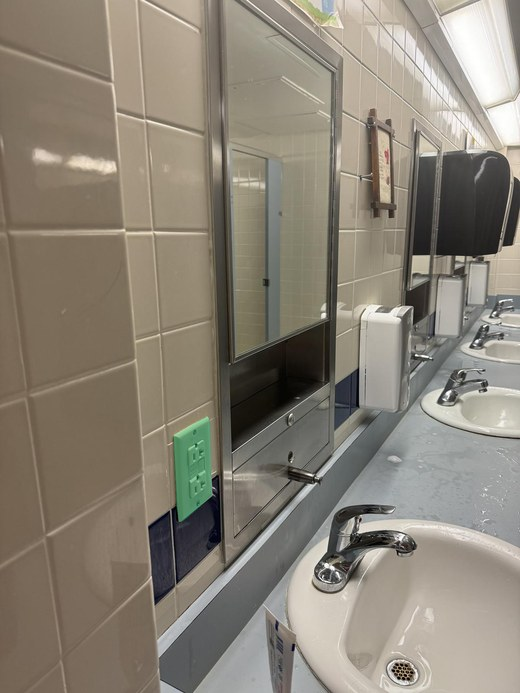
\includegraphics[width=0.26\linewidth]{ex_obs_key.jpg}\hspace{0.02\linewidth}%
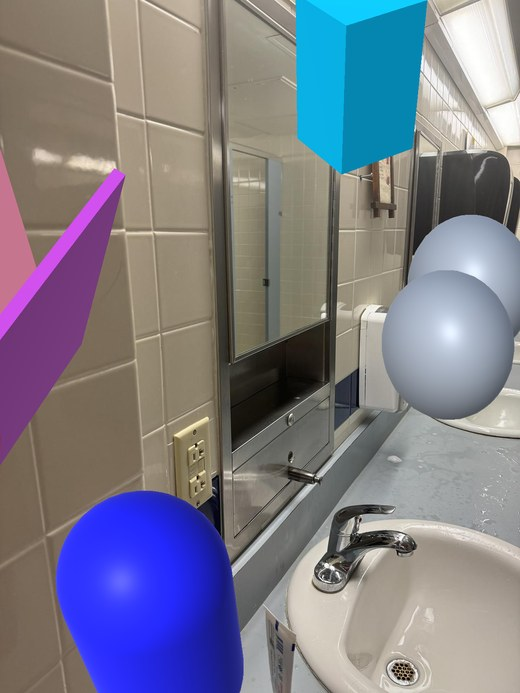
\includegraphics[width=0.26\linewidth]{ex_obs_ar.jpg}\hspace{0.02\linewidth}%
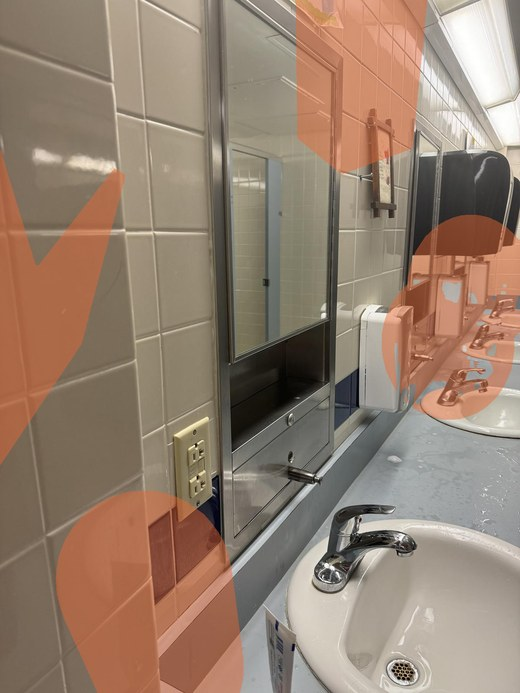
\includegraphics[width=0.26\linewidth]{ex_obs_content.jpg}
\caption{Falso positivo de obstrução (Qwen3-VL-2B, par \texttt{electrical-outlet\_004}). Esquerda:
imagem crua com o objeto-chave verdadeiro (tomada) em verde. Centro: imagem aumentada. Direita: máscara
do conteúdo virtual em laranja. O VLM respondeu ``red box'', exemplo copiado do prompt; a razão de
obstrução do objeto detectado foi 0,45, e o IoU entre a máscara detectada e a verdadeira foi 0,00.}
\label{fig:exobs}
\end{figure}

\subsection{Manipulação: procedimento de atribuição}
Como o dataset traz o rótulo verdadeiro de cada fator, e o VLM responde a cada fator nas perguntas
3--5, cada erro pode ser atribuído a uma causa sem anotação nova. O procedimento tem quatro passos.

\textbf{1. Classificação de cada erro}, nesta ordem:
\begin{itemize}
\item \emph{ilegível}: alguma resposta 3--5 ou a conclusão não pôde ser interpretada;
\item \emph{erro de conclusão}: a conclusão (pergunta 6) contradiz o $A\wedge S\wedge I$ das próprias
  respostas 3--5;
\item \emph{erro de percepção}: a conclusão é coerente, e o erro está nos fatores. Num falso positivo
  coerente, o modelo aceitou os três fatores, então os fatores errados são exatamente os que valem 0. Num
  falso negativo coerente, registra-se o conjunto de fatores verdadeiros que ele rejeitou.
\end{itemize}

\textbf{2. Discriminação por fator.} A taxa de acerto por fator premia o viés para o rótulo
majoritário, que é ``sim'' nos três fatores. Usamos o J de Youden,
$J_F = 1 - P(\text{erro}\mid F=0) - P(\text{erro}\mid F=1)$, que vale 0 quando a resposta não depende
da imagem e 1 quando é perfeita.

\textbf{3. Etapa de conclusão.} Comparamos a decisão do artigo (pergunta 6) com o
$A\wedge S\wedge I$ das respostas 3--5, calculado em código, por McNemar nos mesmos pares.

\textbf{4. Oráculo contrafactual.} Substitui-se a resposta do VLM pela verdade em um fator, mantendo as
outras, e recalcula-se a Eq.~\eqref{eq:man}. A variação da FPR e da FNR é o teto de ganho de qualquer
intervenção que corrija só aquele fator. Um efeito da conjunção precisa ser levado em conta na leitura:
\textbf{um erro num fator só aparece na decisão se os outros dois forem aceitos}. Erros num fator podem
ficar mascarados por erros em outro, e o oráculo os revela.

\subsection{Manipulação: resultados com o prompt do artigo}
As Tabelas~\ref{tab:causas} a~\ref{tab:oraculo} mostram as quatro etapas.

\begin{table}[!t]
\renewcommand{\arraystretch}{1.15}
\caption{Causas dos erros da decisão do artigo (prompt \texttt{paper}). Percepção: fatores aceitos
indevidamente (FP) ou rejeitados indevidamente (FN)}
\label{tab:causas}
\centering
\footnotesize
\fitwidth{%
\begin{tabular}{lcccccccccl}
\toprule
 & \multicolumn{6}{c}{Falsos positivos (de 70)} & \multicolumn{4}{c}{Falsos negativos (de 44)} \\
\cmidrule(lr){2-7}\cmidrule(lr){8-11}
Modelo & Total & Conclusão & só $A$ & só $S$ & só $I$ & $A$ e $S$ & Total & Ilegível & Conclusão & Percepção \\
\midrule
Qwen3-VL-2B & 68 & \textbf{68} & 0 & 0 & 0 & 0 & 2 & 2 & 0 & -- \\
Qwen3-VL-4B & 3 & 0 & 2 & 1 & 0 & 0 & 41 & 0 & 0 & só $I$: \textbf{38}; $A$ e $S$: 3 \\
Qwen3-VL-8B & 70 & \textbf{44} & 10 & 11 & 5 & 0 & 1 & 0 & 0 & $A$, $S$ e $I$: 1 \\
LLaVA-Next-8B & 63 & 0 & \textbf{31} & \textbf{22} & 8 & 2 & 7 & 0 & 0 & $A$ e $S$: 7 \\
Gemma 4 12B & 49 & 0 & \textbf{22} & \textbf{18} & 7 & 2 & 2 & 0 & 1 & só $A$: 1 \\
\midrule
Pares possíveis & 70 & 70 & 32 & 25 & 11 & 2 & 44 & 44 & 44 & 44 \\
\bottomrule
\end{tabular}}
\end{table}

\begin{table}[!t]
\renewcommand{\arraystretch}{1.15}
\caption{Discriminação por fator (J de Youden) no modo conjunto (\texttt{paper}) e no decomposto
(\texttt{paper\_decomposed}). 0 = a resposta não depende da imagem; o J de $I$ usa só 11 negativos}
\label{tab:youden}
\centering
\footnotesize
\begin{tabular}{lcccccc}
\toprule
 & \multicolumn{3}{c}{\texttt{paper}} & \multicolumn{3}{c}{\texttt{paper\_decomposed}} \\
\cmidrule(lr){2-4}\cmidrule(lr){5-7}
Modelo & $J_A$ & $J_S$ & $J_I$ & $J_A$ & $J_S$ & $J_I$ \\
\midrule
Qwen3-VL-2B   & $-0{,}03$ & $-0{,}02$ & 0,00 & $-0{,}03$ & 0,07 & 0,00 \\
Qwen3-VL-4B   & 0,09 & 0,31 & $-0{,}30$ & 0,25 & 0,22 & $-0{,}01$ \\
Qwen3-VL-8B   & \textbf{0,48} & 0,25 & $-0{,}01$ & 0,32 & \textbf{0,50} & $-0{,}09$ \\
LLaVA-Next-8B & $-0{,}13$ & $-0{,}02$ & 0,00 & 0,05 & $-0{,}06$ & 0,00 \\
Gemma 4 12B   & 0,20 & 0,16 & \textbf{0,25} & 0,35 & 0,00 & 0,21 \\
\bottomrule
\end{tabular}
\end{table}

\begin{table}[!t]
\renewcommand{\arraystretch}{1.15}
\caption{Etapa de conclusão: decisão do artigo (Q6) contra $A\wedge S\wedge I$ das respostas 3--5, nas
execuções em que as duas divergem. Nas demais, a coerência fica entre 88\% e 100\%}
\label{tab:conclusao}
\centering
\footnotesize
\fitwidth{%
\begin{tabular}{llccccc}
\toprule
Modelo & Variante & Q6 coerente (\%) & Acurácia: Q6 $\to$ $A\wedge S\wedge I$ & FPR & FNR & $p$ \\
\midrule
Qwen3-VL-2B & \texttt{paper} & 1,8 & 38,6 $\to$ 61,4 & 97,1 $\to$ 0,0 & 4,5 $\to$ 100 & 0,017 \\
Qwen3-VL-8B & \texttt{paper} & 60,5 & 37,7 $\to$ 75,4 & 100 $\to$ 37,1 & 2,3 $\to$ 4,5 & $<0{,}001$ \\
Qwen3-VL-8B & \texttt{neutral} & 69,0 & 60,5 $\to$ \textbf{80,7} & 58,6 $\to$ 17,1 & 9,1 $\to$ 22,7 & $<0{,}001$ \\
Qwen3-VL-8B & \texttt{definition} & 85,1 & 58,8 $\to$ 73,7 & 61,4 $\to$ 37,1 & 9,1 $\to$ 9,1 & $<0{,}001$ \\
LLaVA-Next-8B & \texttt{definition} & 26,3 & 41,2 $\to$ 55,3 & 82,9 $\to$ 11,4 & 20,5 $\to$ 97,7 & 0,10 \\
\bottomrule
\end{tabular}}
\end{table}

\begin{table}[!t]
\renewcommand{\arraystretch}{1.15}
\caption{Oráculo contrafactual no prompt \texttt{paper}: FPR / FNR (\%) com a decisão calculada pela
Eq.~\eqref{eq:man} a partir das respostas 3--5, com a verdade em um ou dois fatores}
\label{tab:oraculo}
\centering
\footnotesize
\begin{tabular}{lccccc}
\toprule
Modelo & Sem oráculo & Oráculo em $A$ & Oráculo em $S$ & Oráculo em $I$ & Oráculo em $A$ e $S$ \\
\midrule
Qwen3-VL-2B   & 0,0 / 100  & 0,0 / 100  & 0,0 / 100  & 84,3 / 4,5 & 0,0 / 100 \\
Qwen3-VL-4B   & 4,3 / 93,2 & 1,4 / 93,2 & 2,9 / 93,2 & \textbf{47,1 / 6,8} & 10,0 / 86,4 \\
Qwen3-VL-8B   & 37,1 / 4,5 & 22,9 / 4,5 & 21,4 / 4,5 & 30,0 / 4,5 & 15,7 / 2,3 \\
LLaVA-Next-8B & 90,0 / 15,9 & \textbf{42,9} / 15,9 & 55,7 / 15,9 & 78,6 / 15,9 & \textbf{15,7 / 0,0} \\
Gemma 4 12B   & 72,9 / 2,3 & \textbf{37,1 / 0,0} & 44,3 / 2,3 & 61,4 / 2,3 & 11,4 / 0,0 \\
\bottomrule
\end{tabular}
\end{table}

\textbf{Não há uma causa comum} (Tabela~\ref{tab:causas}). Os erros do 2B e do 8B vêm sobretudo da
conclusão; os do LLaVA e do Gemma, da aceitação de alinhamento e estilo ruins; os do 4B, da rejeição de
$I$ nos ataques.

\textbf{Dois modelos não percebem os fatores} (Tabela~\ref{tab:youden}). No Qwen3-VL-2B e no LLaVA, o J
fica entre $-0{,}13$ e $+0{,}09$ em todos os fatores e variantes: as respostas não dependem da imagem.
O LLaVA aceita $A$ em 33 dos 34 pares desalinhados e $I$ em todos os pares; chega a descrever ``a cup
of coffee with a saucer, floating above the fan'' na resposta 1 e afirmar, na resposta 3, que o conteúdo
está ``accurately aligned to the fan without a significant gap''. Na família Qwen, o tamanho melhora a
percepção de $A$: $J_A$ vai de $-0{,}03$ (2B) a 0,09 (4B) e 0,48 (8B). \textbf{Nenhum modelo discrimina
$I$}: nas 25 execuções, $J_I$ fica entre $-0{,}30$ e $+0{,}25$, e só o Gemma tem valores positivos em
todas as variantes, com intervalos largos.

\textbf{A conclusão desconectada derruba os modelos que percebem} (Tabela~\ref{tab:conclusao}). O
Qwen3-VL-8B responde ``Yes.'' na pergunta 6 em 113 dos 114 pares, mesmo depois de ``No'' nas perguntas
3 ou 4, como em ``3. No. The virtual plant is positioned floating in the air directly above the hard
drive, with a clear gap [\dots] 6. Yes.''. Aplicando a Eq.~\eqref{eq:man} às mesmas respostas, a
acurácia vai de 37,7\% para 75,4\%; com o prompt \texttt{neutral}, chega a 80,7\%, a única execução do
modo conjunto acima do detector trivial e a mais próxima do GPT-4o. É, no entanto, a melhor de 15
combinações de variante e regra, escolhida depois de ver os dados. No 2B, a conclusão também é
incoerente (coerência de 1,8\%), mas as respostas não salvam o resultado: como ele nega $I$ em todos os
pares, $A\wedge S\wedge I$ nunca dispara e iguala o detector trivial.

\textbf{Nenhum fator corrigido sozinho leva a um bom detector} (Tabela~\ref{tab:oraculo}). No LLaVA e no
Gemma, $A$ é o fator de maior ganho (FPR de 90,0\% para 42,9\% e de 72,9\% para 37,1\%), porque o
desalinhamento é o tipo de negativo mais comum; só corrigindo $A$ e $S$ juntos a FPR cairia para
15,7\% e 11,4\%. No Qwen3-VL-4B, $I$ explica os falsos negativos, mas esconde outros erros: com $I$
correto, a FNR cai de 93,2\% para 6,8\%, e a FPR sobe para 47,1\%, porque os pares desalinhados que o
modelo aceita (65\%) deixam de ser bloqueados pela rejeição de $I$. A FPR baixa desse modelo não é
mérito, mas consequência de rejeitar $I$: ele trata adições plausíveis como inofensivas (``It is a
plausible accessory that enhances the scooter's utility''), enquanto o ViDDAR define o contrário, já que
é a plausibilidade que engana o usuário.

\begin{figure}[!t]
\centering
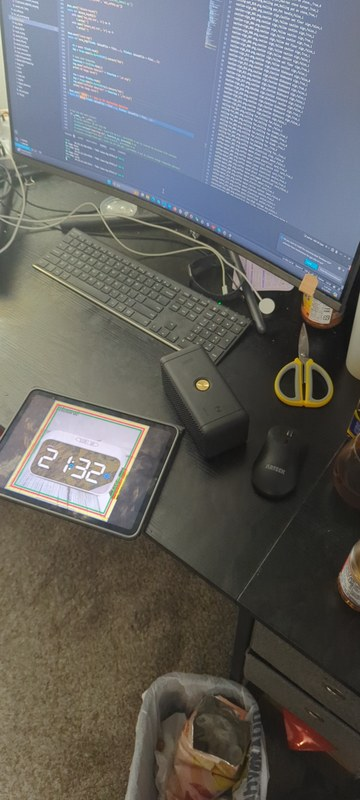
\includegraphics[width=0.24\linewidth]{ex_man_raw.jpg}\hspace{0.03\linewidth}%
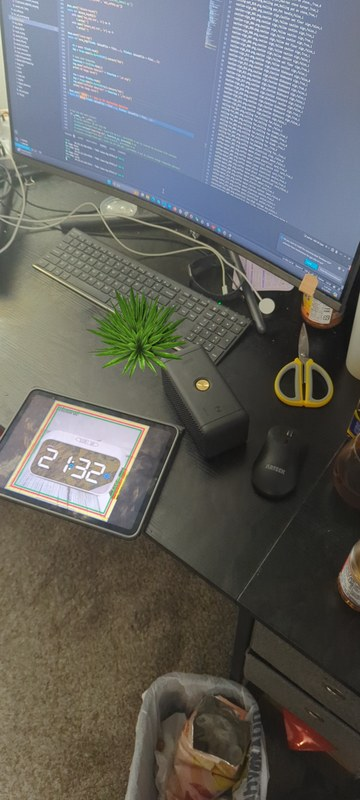
\includegraphics[width=0.24\linewidth]{ex_man_ar.jpg}
\caption{Falso positivo de manipulação (LLaVA-Next-8B, par 2). Esquerda: imagem crua. Direita: imagem
aumentada, com uma planta virtual desalinhada da caixa de som (rótulo $A=0$, $M=0$). A resposta do
modelo começa com ``The virtual content in the augmented image is a digital clock\dots'': ele tomou o
relógio exibido na tela do iPad usado como marcador de calibração, um objeto real, pelo conteúdo
virtual, e o julgou alinhado, realista e enganoso.}
\label{fig:exman}
\end{figure}

\subsection{Manipulação: o que as intervenções mostram}
\label{sec:hipoteses}

\textbf{H1, viés de ``sim'' induzido pelo prompt: confirmada nos modelos que disparam demais.} Com o
\texttt{neutral}, a FPR cai em todos eles: 97\% $\to$ 79\% no 2B, 100\% $\to$ 59\% no 8B, 90\% $\to$
50\% no LLaVA e 70\% $\to$ 41\% no Gemma. A acurácia sobe com significância no 2B, no 8B e no LLaVA. Mas,
nos modelos que não percebem os fatores, a queda de falsos positivos vira aumento de falsos negativos (no
LLaVA, a FNR vai de 15,9\% para 40,9\%), e no 4B, que já quase não disparava, o prompt neutro o leva a
nunca disparar.

\textbf{H2, conclusão desconectada e contaminação entre respostas: confirmada em parte.} Decompor elimina
os erros de conclusão e dá os maiores ganhos do benchmark: +12,3 pontos no 4B, +31,6 e +37,7 no 8B,
+24,6 no LLaVA. Mas cada fator perguntado isoladamente revela um viés próprio, que varia por modelo: o 4B
e o Gemma passam a rejeitar $S$ (o Gemma descreve o conteúdo como ``a 2D sticker placed over the image''
em todos os pares e vira um detector que nunca dispara), e o LLaVA passa a rejeitar $A$ nos ataques. O
julgamento de $S$ do Gemma depende mais da forma da pergunta do que da imagem.

\textbf{H3, leitura restritiva de $I$: não confirmada como uma leitura melhor de $I$.} No modo conjunto,
a definição tem efeitos em direções opostas: o 4B passa a disparar mais em todos os fatores, o LLaVA
desconecta a conclusão (coerência de 26\%), e o ganho do 8B vem da conclusão, não de $I$. No 8B
decomposto, a definição tem efeito significativo (+6,1 pontos sobre \texttt{paper\_decomposed},
$p=0{,}016$), e os falsos negativos por $I$ somem (7 $\to$ 0); mas $J_I$ não sobe ($-0{,}09$ $\to$
0,00): o modelo passa a aceitar $I$ em todos os pares. O ganho vem de $I=1$ ser majoritário no
dataset (103 de 114 pares), não de uma interpretação melhor.

\textbf{C2, alinhamento geométrico: confirmado no nível do fator, não da decisão}
(Tabela~\ref{tab:c2}). A medida geométrica julga $A$ melhor que o VLM em 9 de 10 execuções, com AUC de
0,65 a 0,80. Mas, isolando o efeito geométrico (comparando o híbrido com o $A\wedge S\wedge I$ do próprio
VLM, que só difere em $A$), só o LLaVA \texttt{paper} melhora com significância, e por troca: a FPR cai
de 90\% para 41\%, e a FNR sobe de 16\% para 57\%. Os saltos do 2B e do 8B no \texttt{paper} vêm de
trocar a pergunta 6 pela regra, e não da geometria. Um $A$ melhor não ajuda porque a decisão é uma
conjunção: onde $S$ ou $I$ já bloqueiam o ataque, $A$ não importa; onde o VLM aceita tudo, a geometria
corta falsos positivos, mas também ataques, porque a própria medida erra de 20\% a 40\% dos pares.

\begin{table}[!t]
\renewcommand{\arraystretch}{1.15}
\caption{Alinhamento geométrico (C2) no prompt \texttt{paper} e na melhor variante de cada modelo.
Acerto em $A$ e acurácias em \%; $p$ de McNemar do híbrido contra $A\wedge S\wedge I$ do VLM}
\label{tab:c2}
\centering
\footnotesize
\fitwidth{%
\begin{tabular}{llccccc}
\toprule
Modelo & Variante & Acerto em $A$: geometria / VLM & AUC & Q6 $\to$ híbrido & $A\wedge S\wedge I$ $\to$ híbrido & $p$ \\
\midrule
Qwen3-VL-2B & \texttt{paper} & 79 / 70 & 0,79 & 38,6 $\to$ 61,4 & 61,4 $\to$ 61,4 & 1,00 \\
 & \texttt{neutral} & 79 / 70 & 0,80 & 48,2 $\to$ 60,5 & 60,5 $\to$ 60,5 & 1,00 \\
Qwen3-VL-4B & \texttt{paper} & 76 / 62 & 0,72 & 61,4 $\to$ 61,4 & 61,4 $\to$ 61,4 & 1,00 \\
 & \texttt{paper\_decomposed} & 76 / 63 & 0,72 & 73,7 $\to$ 71,1 & 73,7 $\to$ 71,1 & 0,25 \\
Qwen3-VL-8B & \texttt{paper} & 80 / 75 & 0,76 & 37,7 $\to$ 78,1 & 75,4 $\to$ 78,1 & 0,58 \\
 & \texttt{definition\_decomposed} & 75 / 74 & 0,75 & 75,4 $\to$ 75,4 & 75,4 $\to$ 75,4 & 1,00 \\
LLaVA-Next-8B & \texttt{paper} & 65 / 60 & 0,72 & 38,6 $\to$ 52,6 & 38,6 $\to$ \textbf{52,6} & \textbf{0,036} \\
 & \texttt{paper\_decomposed} & 59 / 41 & 0,65 & 63,2 $\to$ 62,3 & 63,2 $\to$ 62,3 & 1,00 \\
Gemma 4 12B & \texttt{paper} & 73 / 74 & 0,70 & 55,3 $\to$ 59,6 & 54,4 $\to$ 59,6 & 0,36 \\
 & \texttt{definition} & 75 / 69 & 0,72 & 63,2 $\to$ 65,8 & 61,4 $\to$ 65,8 & 0,46 \\
\bottomrule
\end{tabular}}
\end{table}

A Tabela~\ref{tab:problemas} resume os mecanismos e o efeito de cada intervenção.

\begin{table}[!t]
\renewcommand{\arraystretch}{1.2}
\caption{Mecanismos de erro na manipulação e efeito das intervenções}
\label{tab:problemas}
\centering
\footnotesize
\begin{tabular}{L{4.4cm}L{3.0cm}L{8.4cm}}
\toprule
Mecanismo & Onde aparece & Intervenção e efeito \\
\midrule
P1. Conclusão que contradiz as próprias respostas & Qwen3-VL-2B e 8B; LLaVA com \texttt{definition} & decisão calculada fora do VLM (modo decomposto ou $A\wedge S\wedge I$): elimina o erro e dá os maiores ganhos, mas só no modelo que percebe os fatores (8B) \\
P2. Viés de ``sim'' e percepção fraca de $A$ e $S$ & LLaVA, Gemma; 2B & prompt neutro: reduz a FPR, mas troca FP por FN nos modelos com $J\approx 0$; alinhamento geométrico: mede $A$ melhor, sem ganho na decisão \\
P3. Leitura errada de $I$: restritiva (FN) ou trivial (FP) & Qwen3-VL-4B; LLaVA & definição explícita de $I$: os modelos passam a aceitar $I$ sempre, sem discriminá-lo \\
\bottomrule
\end{tabular}
\end{table}

% =====================================================================================================
\section{Discussão}
\label{sec:disc}

\textbf{A replicação é confiável.} Os componentes sem VLM reproduzem o artigo quase exatamente, e o
mesmo VLM do artigo produz números próximos dos publicados nas duas tarefas. As diferenças entre
modelos podem, portanto, ser atribuídas aos modelos, e não à reimplementação.

\textbf{O que protege o detector é tirar a decisão do VLM.} O padrão atravessa as duas tarefas. Na
obstrução, em que o VLM só nomeia um objeto e a geometria decide, modelos abertos a partir de 4B
parâmetros chegam ao nível do GPT-4o e do limite superior do pipeline; quando o VLM decide sozinho
(\emph{end-to-end}), cada modelo exibe o próprio viés de ``sim'' ou ``não''. Na manipulação, em que o
VLM decide tudo, nenhum modelo supera o detector trivial com o prompt do artigo, e os melhores
resultados vieram justamente de calcular a decisão fora dele. Para modelos pequenos, a divisão de
trabalho entre o VLM, que reconhece, e uma regra explícita, que decide, importa mais que o tamanho do
modelo.

\textbf{Tirar a decisão do VLM só ajuda quem percebe.} Os únicos casos em que os falsos positivos da
manipulação caíram sem custar quase todos os ataques foram no Qwen3-VL-8B, em que se juntaram uma
percepção mínima dos fatores ($J>0$ em $A$ e $S$) e a decisão fora da etapa de conclusão. Nos modelos com
$J\approx 0$, toda intervenção apenas desloca o viés, trocando falsos positivos por falsos negativos. A
escala ajuda a percepção dentro da família Qwen, mas isso só aparece na acurácia quando a conclusão sai
do VLM.

\textbf{Acurácia não basta.} Com 70 benignos e 44 ataques, o detector que nunca dispara acerta 61,4\%,
e na obstrução e na manipulação há modelos que atingem acurácias parecidas por caminhos opostos.
Comparar detectores exige reportar FPR e FNR, compará-los ao detector trivial e, quando possível,
decompor os erros. A composição do dataset agrava o problema: como os negativos da manipulação são
``quase ataques'', com dois fatores verdadeiros, qualquer viés de ``sim'' se converte diretamente em
falsos positivos.

\textbf{O fator semântico não é medido de forma confiável.} Nenhum modelo discrimina $I$, que é
justamente o que distingue um ataque de um conteúdo apenas bem encaixado, e as variantes que melhoram o
resultado o fazem aceitando $I$ sempre: na prática, o detector se reduz a $A\wedge S$. O dataset também
não permite medi-lo bem, com só 11 pares benignos em $I$.

\textbf{Os falsos positivos nascem da ambiguidade.} Na obstrução, todos os falsos positivos vêm de cenas
com mais de um objeto relevante, em que o VLM escolhe um candidato razoável diferente do anotado. Na
manipulação, o LLaVA tomou um objeto real pelo conteúdo virtual (Fig.~\ref{fig:exman}). Nos dois casos,
o VLM se fixa num elemento plausível que não é o alvo. Em cenas menos controladas que as do dataset, com
mais objetos e sobreposições já presentes na imagem, esse mecanismo tende a ser mais frequente.

% =====================================================================================================
\section{Limitações e trabalhos futuros}
\label{sec:futuro}

\subsection{Limitações}
\begin{itemize}
\item \textbf{Escolhas depois de ver os dados.} A melhor variante de cada modelo e a regra
  $A\wedge S\wedge I$ foram escolhidas olhando os resultados, sem conjunto de teste separado. Com 25
  execuções e vários testes, algum $p<0{,}05$ pode ser acaso. As variantes foram, porém, escritas a
  partir das definições do artigo, e todas são reportadas.
\item \textbf{Tamanho da amostra.} Com 114 pares de manipulação, só 11 benignos em $I$ e 27 em $S$, os
  intervalos de confiança são largos. Na obstrução, algumas classes têm só 3 a 8 amostras.
\item \textbf{Uma execução por configuração}, com decodificação greedy; não estimamos a variância entre
  execuções, que o próprio artigo aponta como fonte de instabilidade.
\item \textbf{Modelos.} Três dos cinco VLMs rodam em 4 bits, o que pode mudar as respostas em relação
  aos modelos completos, e o Gemma usa um orçamento de tokens por imagem menor que o dos Qwen. Não
  executamos o GPT-4o: a comparação com ele usa os números publicados, sem teste pareado.
\item \textbf{Atribuição.} Depende de extrair as respostas 3--5 do texto livre do VLM. O oráculo é um
  teto contrafactual que supõe as demais respostas fixas. Na obstrução, ``objeto errado'' mistura erros
  do VLM e do detector; a comparação com o \emph{prior knowledge} separa só parte deles.
\item \textbf{Reconstrução.} As máscaras $m_c$ são derivadas por diferença de pixels, o que pode explicar
  o $\alpha$ ótimo de 0,20; o Grounding DINO aberto substitui o 1.5; e nossos critérios de acerto do
  objeto-chave não são diretamente comparáveis com o do artigo, que não foi publicado.
\end{itemize}

\subsection{Trabalhos futuros}
\begin{itemize}
\item \textbf{Validação sem seleção nos dados de teste:} congelar as configurações escolhidas aqui e
  avaliá-las em dados novos, ou separar um subconjunto de desenvolvimento estratificado por
  $(A,S,I)$, e repetir as execuções com amostragem para estimar a variância.
\item \textbf{O fator $I$:} ampliar os negativos em $I$ e investigar formas de medir esse fator que não
  dependam de um ``sim'' ou ``não'' do VLM.
\item \textbf{Definição do objeto-chave:} na obstrução, especificar no prompt ou no rótulo como resolver
  cenas com mais de um objeto relevante, que concentram os falsos positivos.
\item \textbf{Cenas menos controladas:} avaliar a robustez dos detectores a condições reais da cena, como
  degradação física de objetos e sobreposições já presentes na imagem, que podem ser tomadas por
  conteúdo virtual.
\item \textbf{Execução na borda:} medir latência e consumo dos modelos de 4B, que já bastam para a
  obstrução, em hardware de borda.
\end{itemize}

% =====================================================================================================
\section{Conclusão}
Reconstruímos e validamos o pipeline de avaliação do ViDDAR e o avaliamos com cinco VLMs abertos
executados localmente. Na detecção de obstrução, em que a decisão final é geométrica, modelos a partir
de 4B parâmetros chegam ao nível do GPT-4o, e os poucos falsos positivos vêm da ambiguidade sobre qual
objeto importa. Na detecção de manipulação, em que o VLM decide sozinho, nenhum modelo supera o detector
trivial com o prompt do artigo. Os procedimentos de atribuição propostos, que usam apenas os rótulos do
próprio dataset, mostram que os modelos erram por mecanismos distintos e que cada intervenção resolve
uma parte do problema: tirar a decisão do VLM corrige a conclusão desconectada, mas só ajuda os modelos
que percebem os fatores; o prompt neutro e o alinhamento geométrico deslocam o viés sem melhorar a
decisão; e nenhum modelo discrimina o fator semântico que define o ataque.

% =====================================================================================================
\begin{thebibliography}{99}

\bibitem{viddar}
Y.~Xiu, T.~Scargill, and M.~Gorlatova, ``{ViDDAR}: Vision language model-based task-detrimental
content detection for augmented reality,'' \emph{IEEE Trans. Vis. Comput. Graphics}, vol.~31, no.~5,
pp. 3194--3203, 2025, doi: 10.1109/TVCG.2025.3549147.

\bibitem{vimsense}
Y.~Xiu and M.~Gorlatova, ``Detecting visual information manipulation attacks in augmented reality: A
multimodal semantic reasoning approach,'' \emph{IEEE Trans. Vis. Comput. Graphics}, 2025, preprint
arXiv:2507.20356.

\bibitem{lobstar}
Y.~Xiu, T.~Scargill, and M.~Gorlatova, ``{LOBSTAR}: Language model-based obstruction detection for
augmented reality,'' in \emph{Proc. IEEE Int. Symp. Mixed Augmented Reality Adjunct (ISMAR-Adjunct)},
2024.

\bibitem{sabelman2015}
E.~E. Sabelman and R.~Lam, ``The real-life dangers of augmented reality,'' \emph{IEEE Spectrum},
vol.~52, no.~7, pp. 48--53, 2015.

\bibitem{lebeck2017}
K.~Lebeck, K.~Ruth, T.~Kohno, and F.~Roesner, ``Securing augmented reality output,'' in \emph{Proc.
IEEE Symp. Security Privacy (SP)}, 2017, pp. 320--337.

\bibitem{lebeck2018}
K.~Lebeck, K.~Ruth, T.~Kohno, and F.~Roesner, ``Arya: Operating system support for securely augmenting
reality,'' \emph{IEEE Security \& Privacy}, vol.~16, no.~1, pp. 44--53, 2018.

\bibitem{davari2020}
S.~Davari, F.~Lu, and D.~A. Bowman, ``Occlusion management techniques for everyday glanceable {AR}
interfaces,'' in \emph{Proc. IEEE Conf. Virtual Reality 3D User Interfaces Abstracts Workshops (VRW)},
2020.

\bibitem{cheng2023}
K.~Cheng, J.~F. Tian, T.~Kohno, and F.~Roesner, ``Exploring user reactions and mental models towards
perceptual manipulation attacks in mixed reality,'' in \emph{Proc. USENIX Security Symp.}, 2023.

\bibitem{wang2024}
X.~Wang, L.-H. Lee, C.~Bermejo Fernandez, and P.~Hui, ``The dark side of augmented reality: Exploring
manipulative designs in {AR},'' \emph{Int. J. Human--Computer Interaction}, vol.~40, no.~13,
pp. 3449--3464, 2024.

\bibitem{duan2022}
H.~Duan, X.~Min, Y.~Zhu, G.~Zhai, X.~Yang, and P.~Le~Callet, ``Confusing image quality assessment:
Toward better augmented reality experience,'' \emph{IEEE Trans. Image Process.}, vol.~31,
pp. 7206--7221, 2022.

\bibitem{duan2025}
L.~Duan, Y.~Xiu, and M.~Gorlatova, ``Advancing the understanding and evaluation of {AR}-generated
scenes: When vision-language models shine and stumble,'' in \emph{Proc. IEEE Conf. Virtual Reality 3D
User Interfaces Abstracts Workshops (VRW)}, 2025.

\bibitem{tong2024}
S.~Tong, Z.~Liu, Y.~Zhai, Y.~Ma, Y.~LeCun, and S.~Xie, ``Eyes wide shut? {E}xploring the visual
shortcomings of multimodal {LLMs},'' in \emph{Proc. IEEE/CVF Conf. Comput. Vis. Pattern Recognit.
(CVPR)}, 2024, pp. 9568--9578.

\bibitem{guan2024}
T.~Guan \emph{et al.}, ``{HallusionBench}: An advanced diagnostic suite for entangled language
hallucination and visual illusion in large vision-language models,'' in \emph{Proc. IEEE/CVF Conf.
Comput. Vis. Pattern Recognit. (CVPR)}, 2024, pp. 14375--14385.

% VERIFICAR: referência nova, não citada pelo ViDDAR nem pelo VIM-Sense; conferir dados bibliográficos.
\bibitem{pope2023}
Y.~Li, Y.~Du, K.~Zhou, J.~Wang, W.~X. Zhao, and J.-R. Wen, ``Evaluating object hallucination in large
vision-language models,'' in \emph{Proc. Conf. Empirical Methods Natural Lang. Process. (EMNLP)}, 2023.

\bibitem{groundingdino}
S.~Liu \emph{et al.}, ``Grounding {DINO}: Marrying {DINO} with grounded pre-training for open-set
object detection,'' in \emph{Proc. Eur. Conf. Comput. Vis. (ECCV)}, 2024, preprint arXiv:2303.05499.

\bibitem{sam}
A.~Kirillov \emph{et al.}, ``Segment anything,'' in \emph{Proc. IEEE/CVF Int. Conf. Comput. Vis.
(ICCV)}, 2023, pp. 4015--4026.

\bibitem{llava}
H.~Liu, C.~Li, Q.~Wu, and Y.~J. Lee, ``Visual instruction tuning,'' in \emph{Adv. Neural Inf.
Process. Syst. (NeurIPS)}, vol.~36, 2023.

\bibitem{qwen3vl}
Qwen Team, ``{Qwen3-VL} model cards (2B, 4B and 8B Instruct),'' Hugging Face, 2025. [Online].
Available: \url{https://huggingface.co/Qwen/Qwen3-VL-4B-Instruct}

% VERIFICAR: citar o relatório técnico do Gemma 4, se houver; por ora, o model card.
\bibitem{gemma4}
Gemma Team, Google, ``{Gemma 4} model card (12B instruction-tuned),'' Hugging Face. [Online].
Available: \url{https://huggingface.co/google/gemma-4-12B-it}

\bibitem{qlora}
T.~Dettmers, A.~Pagnoni, A.~Holtzman, and L.~Zettlemoyer, ``{QLoRA}: Efficient finetuning of
quantized {LLMs},'' in \emph{Adv. Neural Inf. Process. Syst. (NeurIPS)}, vol.~36, 2023.

\bibitem{hou2007}
X.~Hou and L.~Zhang, ``Saliency detection: A spectral residual approach,'' in \emph{Proc. IEEE Conf.
Comput. Vis. Pattern Recognit. (CVPR)}, 2007.

\bibitem{canny}
J.~Canny, ``A computational approach to edge detection,'' \emph{IEEE Trans. Pattern Anal. Mach.
Intell.}, vol.~PAMI-8, no.~6, pp. 679--698, 1986.

\bibitem{wilson}
E.~B. Wilson, ``Probable inference, the law of succession, and statistical inference,'' \emph{J. Amer.
Statist. Assoc.}, vol.~22, no.~158, pp. 209--212, 1927.

\end{thebibliography}

\end{document}
